\documentclass{article}\usepackage[]{graphicx}\usepackage[]{color}
% maxwidth is the original width if it is less than linewidth
% otherwise use linewidth (to make sure the graphics do not exceed the margin)
\makeatletter
\def\maxwidth{ %
  \ifdim\Gin@nat@width>\linewidth
    \linewidth
  \else
    \Gin@nat@width
  \fi
}
\makeatother

\definecolor{fgcolor}{rgb}{0.345, 0.345, 0.345}
\newcommand{\hlnum}[1]{\textcolor[rgb]{0.686,0.059,0.569}{#1}}%
\newcommand{\hlstr}[1]{\textcolor[rgb]{0.192,0.494,0.8}{#1}}%
\newcommand{\hlcom}[1]{\textcolor[rgb]{0.678,0.584,0.686}{\textit{#1}}}%
\newcommand{\hlopt}[1]{\textcolor[rgb]{0,0,0}{#1}}%
\newcommand{\hlstd}[1]{\textcolor[rgb]{0.345,0.345,0.345}{#1}}%
\newcommand{\hlkwa}[1]{\textcolor[rgb]{0.161,0.373,0.58}{\textbf{#1}}}%
\newcommand{\hlkwb}[1]{\textcolor[rgb]{0.69,0.353,0.396}{#1}}%
\newcommand{\hlkwc}[1]{\textcolor[rgb]{0.333,0.667,0.333}{#1}}%
\newcommand{\hlkwd}[1]{\textcolor[rgb]{0.737,0.353,0.396}{\textbf{#1}}}%
\let\hlipl\hlkwb

\usepackage{framed}
\makeatletter
\newenvironment{kframe}{%
 \def\at@end@of@kframe{}%
 \ifinner\ifhmode%
  \def\at@end@of@kframe{\end{minipage}}%
  \begin{minipage}{\columnwidth}%
 \fi\fi%
 \def\FrameCommand##1{\hskip\@totalleftmargin \hskip-\fboxsep
 \colorbox{shadecolor}{##1}\hskip-\fboxsep
     % There is no \\@totalrightmargin, so:
     \hskip-\linewidth \hskip-\@totalleftmargin \hskip\columnwidth}%
 \MakeFramed {\advance\hsize-\width
   \@totalleftmargin\z@ \linewidth\hsize
   \@setminipage}}%
 {\par\unskip\endMakeFramed%
 \at@end@of@kframe}
\makeatother

\definecolor{shadecolor}{rgb}{.97, .97, .97}
\definecolor{messagecolor}{rgb}{0, 0, 0}
\definecolor{warningcolor}{rgb}{1, 0, 1}
\definecolor{errorcolor}{rgb}{1, 0, 0}
\newenvironment{knitrout}{}{} % an empty environment to be redefined in TeX

\usepackage{alltt}
\usepackage[a4paper,
            bindingoffset=0.2in,
            left=0.3in,
            right=0.3in,
            top=1in,
            bottom=1in,
            footskip=.25in]{geometry}
\IfFileExists{upquote.sty}{\usepackage{upquote}}{}
\begin{document}

\section{Relationship between Unemployment Gap and Inflation since 04-2020}

\begin{knitrout}
\definecolor{shadecolor}{rgb}{0.969, 0.969, 0.969}\color{fgcolor}
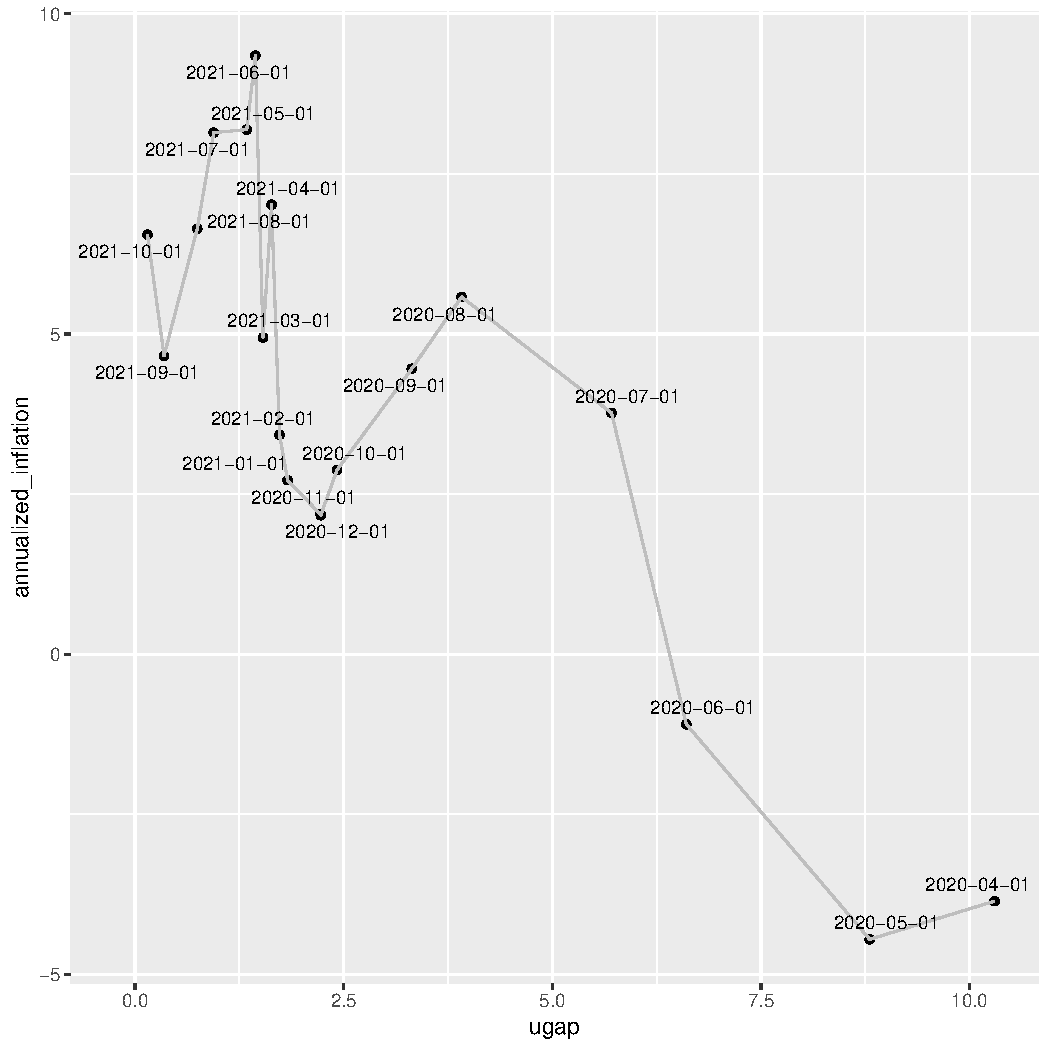
\includegraphics[width=\maxwidth]{figure/unnamed-chunk-1-1} 

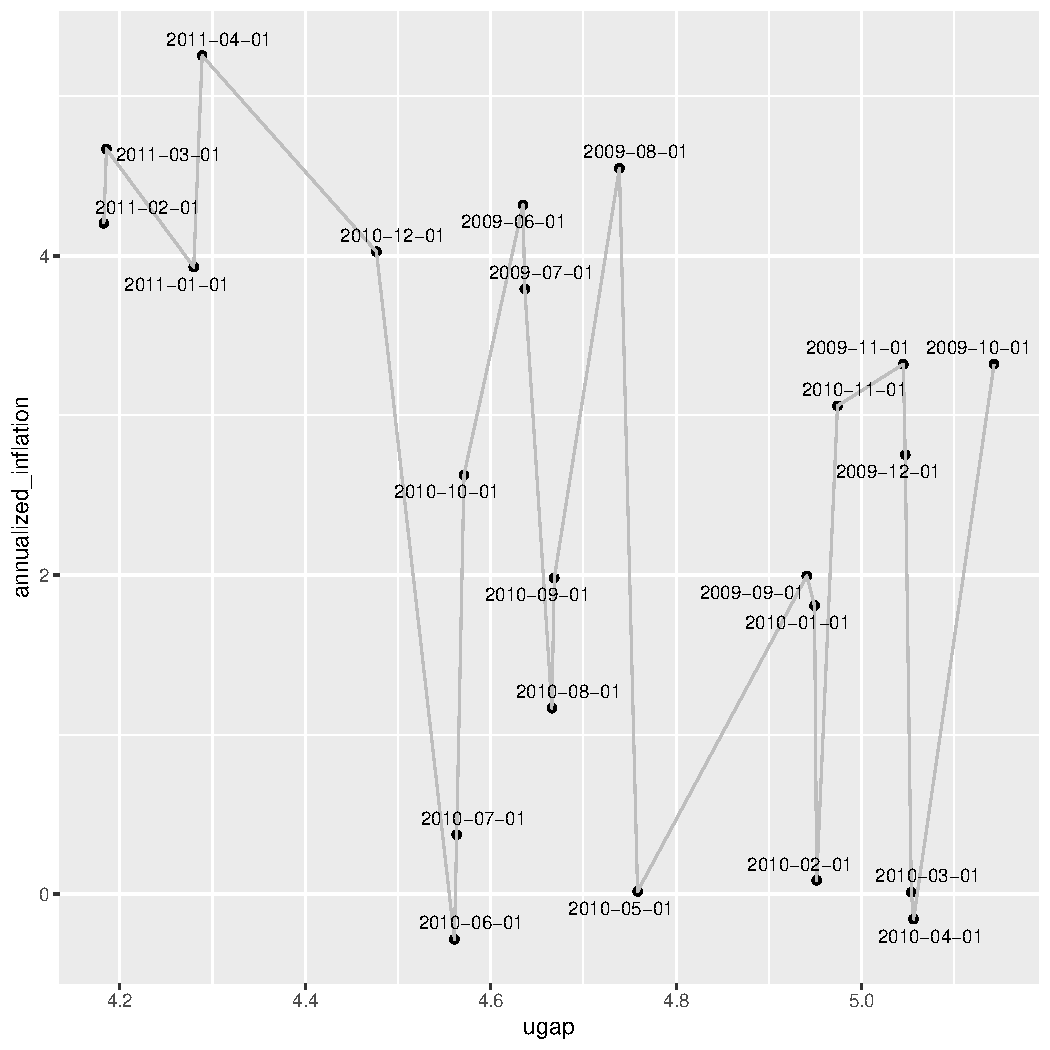
\includegraphics[width=\maxwidth]{figure/unnamed-chunk-1-2} 

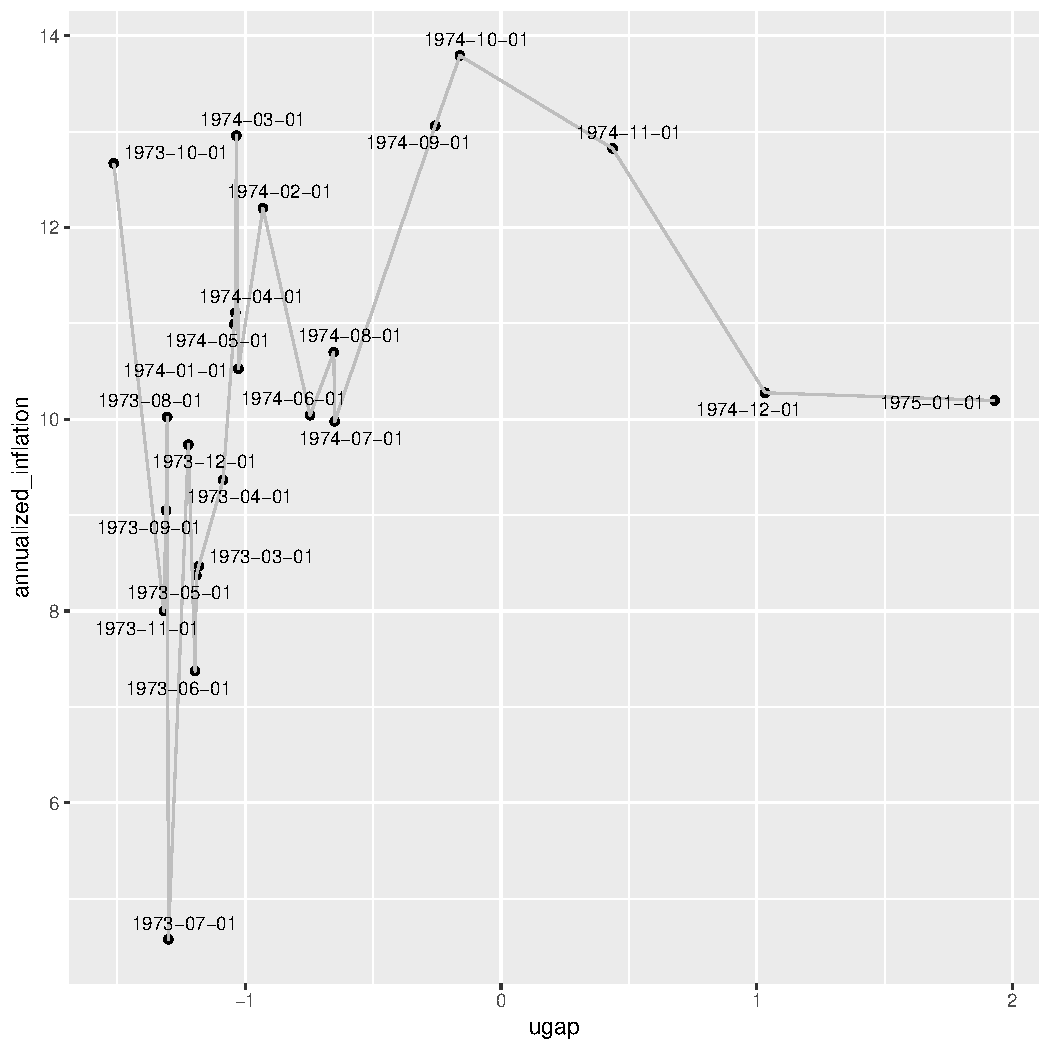
\includegraphics[width=\maxwidth]{figure/unnamed-chunk-1-3} 

\end{knitrout}

The first graph depicts the aftermath of the official COVID-19 recession, which lasted according to the NBER from 2020-02 to 2020-04. The graph indicates that there is an inverse relationship between the unemployment gap and the inflation rate, as suggested by the Phillips Curve. It seems as if the slope gets steeper, when inflation is in generally higher. Evidence shows that the slope flattens in low inflation environments as well as during recessions. However, it is somewhat weird that both inflation and unemployment decreases between 2020-08 and 2021-03. \\

Hypothesis 1: The slope of the Phillips Curve gets steeper in the aftermath of the official Pandemic recession (compared to the beginning of the same period).  \\

The second graph depicts the aftermath (2 years) after the Great Recession. The graph indicates that there is merely a (inverse) relationship between the unemployment gap and the inflation rate. Inflation seems rather driven by other factors, thus the slope of the Phillips Curve during that period must be really small. It must be noted though, that both inflation and unemployment gap do not reaches values as high as in the COVID case. \\

The third graph depicts 2 years during the Great Inflation in order to assess the relationship in a high-inflation environment. The graph indicates a initially recognizable but then missing inverse relationship. 

(Hypothesis 2: The steeper slope in the aftermath of the official Pandemic recession is more likely to be driven by the high inflation than by the "after recession characteristics". Can we compare the different types of recessions?) 

\begin{knitrout}
\definecolor{shadecolor}{rgb}{0.969, 0.969, 0.969}\color{fgcolor}
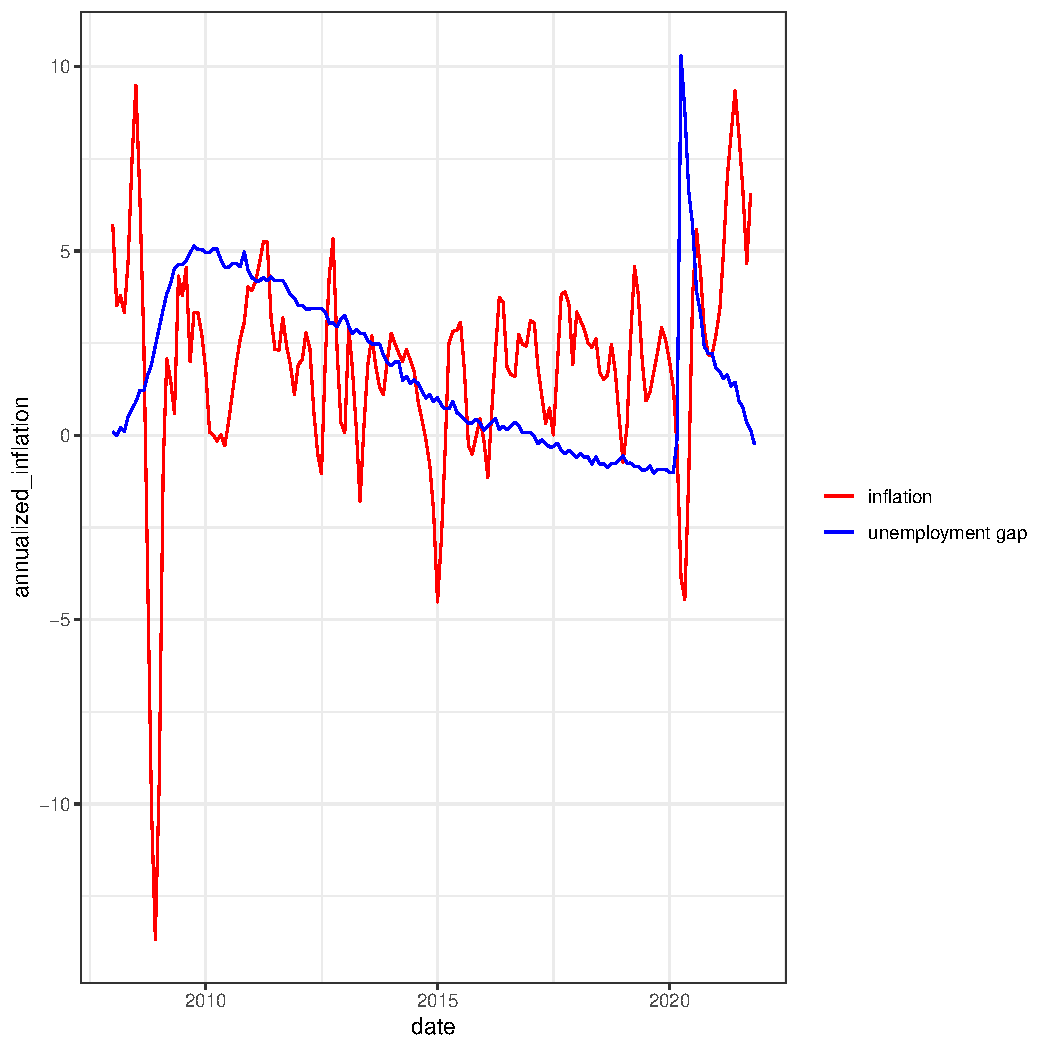
\includegraphics[width=\maxwidth]{figure/unnamed-chunk-2-1} 

\end{knitrout}

This graph shows the co-movement of inflation and the unemployment gap since the beginning of 2008. First, the graph indicates that inflation reacted stronger to the unemployment gap in the aftermath of the COVID recession compared to the same recession itself, i.e. a less steep decrease in the unemployment gap induced a relatively larger increase in the inflation rate (Hypothesis 1). Second, the graph indicates that inflation reacted stronger to the increase in the unemployment gap during the financial crisis than during the COVID recession, which means that the slope of the Phillips Curve must be larger during the 2008 recession compared to the more recent one. \\

Hypothesis 2: The slope during the Financial Crisis is larger than the slope during the COVID recession. \\

When we stop the observations right after the COVID recession, i.e. 2020-04, the overall picture would reflect the evidence of a flattened Phillips Curve. However, the suggested stronger relationship in its aftermath somewhat contradicts that view. What factors can explain the seemingly stronger relationship after the outbreak of the pandemic? Or is the co-movement rather a coincidence, i.e. does the unemployment gap just slowly return to a pre-crisis level and is inflation driven by other factors, such as higher inflation expectations (increased inflation salience, high price volatilities of frequently used products and services), pandemic-owed supply shocks etc.?


Why has (core) inflation not fallen further during the COVID recession? 
Why has (core) inflation risen after the COVID recession? 



\end{document}
